\section{Variational Autoencoder}\raggedbottom
Variational Autoencoder \citep{kingma2014autoencoding} gehören zu den probabilistischen generativen Modelarchitekturen. In den letzten Jahren haben generative Modelle, insbesondere auch Variational Autoencoder, beeindruckende Möglichkeiten aufgezeigt, um hochrealistische Daten wie zum Beispiel Bilder, Text oder Audios zu generieren.
Generative Modelle versuchen die Merkmale und Verteilung eines Datensatzes zu verstehen und anschließend neuartige Datenbeispiele, die ähnlich zum Trainingsdatensatz sind zu generieren.

Normale Autoencoder bestehen aus einem Encoder und einem Decoder, wobei der Encoder versucht eine komprimierte Darstellung $c\in \mathbb{R}^m$ für die Eingabedaten $x\in \mathbb{R}^n$ im Latentspace zu finden. Die komprimierte Darstellung im Latentspace wird vom Decoder rekonstruiert mit dem Ziel eine möglichst identische Rekonstruktion zur Eingabe $x\in \mathxbb{R}^n$ zu erzeugen.
Autoencoder erzeugen nur einen diskreten Latentraum, wodurch Interpolation durch den Latentraum um neue Ausgaben zu rekonstruieren nicht möglich ist, da im Latentraum viele leere Stellen existieren.

Im Gegensatz zu normalen Autoencodern verwenden Variational Autoencoder einen probabilistischen Ansatz um Datenpunkte $x$ im Latentspace $Z$ zu repräsentieren. Das Ziel des Variational Autoencoder ist es, eine multivariate Verteilung zu Der Encoder encodieren Variational Autoencoder die Eingangsdaten in eine multivariate latente Verteilung.e um so einen kontinuierlichen Latentraum zu erzeugen.
Somit kann in diesem Latentraum zwischen den einzelnen Datenpunkten interpoliert werden.


\subsection{ELBO}


\subsection{Cyclical Annealing Schedule}
\label{cyc_anneal}
sonst erklärung unten bei optimus

\subsection{Optimus}
Optimus (\textbf{O}rganizing \textbf{S}entences via \textbf{P}re-trained \textbf{M}odeling of a \textbf{L}atent \textbf{S}pace) \citep{DBLP:journals/corr/abs-2004-04092} ist ein großes vortrainiertes Deep Latent Variable Model für natürliche Sprache.
Die Modelarchitektur von Optimus ist ein Variational Autoencoder, der als Encoder BERT und als Decoder GPT-2 verwendet wie in Abbildung \ref{optimus_scheme_fig} zu erkennen ist. 
Verwendet wird jeweils das vortrainierte BERT Base Modell $\phi_{BERT}$ und das vortrainierte GPT-2 Base Modell $\theta_{GPT-2}$ beide mit 12 Layern, 12 Attention Heads und einer Hiddensize von 768. 
\begin{figure}[h]
    \centering
    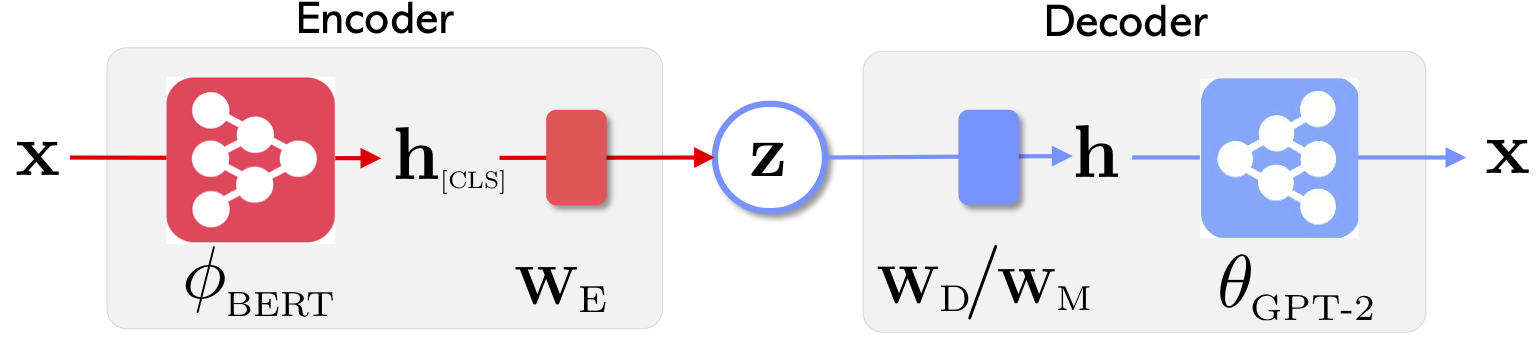
\includegraphics[width=\textwidth]{bilder/optimus_scheme}
    \caption{VAE Modellarchitektur von OPTIMUS mit BERT als Encoder und GPT-2 als Decoder}
    \label{optimus_scheme_fig}
\end{figure}
Trainiert wird Optimus mit dem Ziel Sätze in einen universellen Latentspace zu organisieren und somit übergreifende semantische Muster für die einzelnen Sätze zu finden.
Somit kann durch gezieltes Verändern des Latentvektors $z$ kontrolliert Text generiert werden. ÜBERARBEITEN

BERT und GPT-2 über eine VAE Architektur miteinander zu verbinden hat die Herausforderung die unterschiedlichen Tokenisierungsschemen der einzelnen Modelle zu verwenden und den Latentvektor bei der Textgeneration von GPT-2 zu injizieren. 
Die Eingabetokens von BERT verwenden das WordPiece Embeddings verfahren mit einer Vokabulargröße von 28.996. Die Ausgabe erfolge über die Byte Pair Encoding Tokenisierung von GPT-2 mit einer Vokabulargröße von 50.260. Innerhalb des Netzwerkes wird im Latentvektor ein Token durch eine Einbettung $h_{Emb}$ die das Token, die Position und das Segment Embedding wiedergibt, repräsentiert.
Um beim Training den Loss des Rekonstruktionstask zu berechnen, werden die Sätze mit beiden Tokenisierungen tokenisiert.

Als Latentvektor $z \in \mathbb{R}^P$ wird die gepoolte Ausgabe des letzten Hiddenlayers $h_{[CLS]} \in \mathbb{R}^H$ von BERT multipliziert mit einer Gewichtsmatrix $W_{E} \in \mathbb{R}^{P\times H}$ gewählt. Somit kann ein Latentvektor wie folgt bestimmt werden $z = W_{E}h_{[CLS]}$.

\begin{figure}[h]
    \centering
    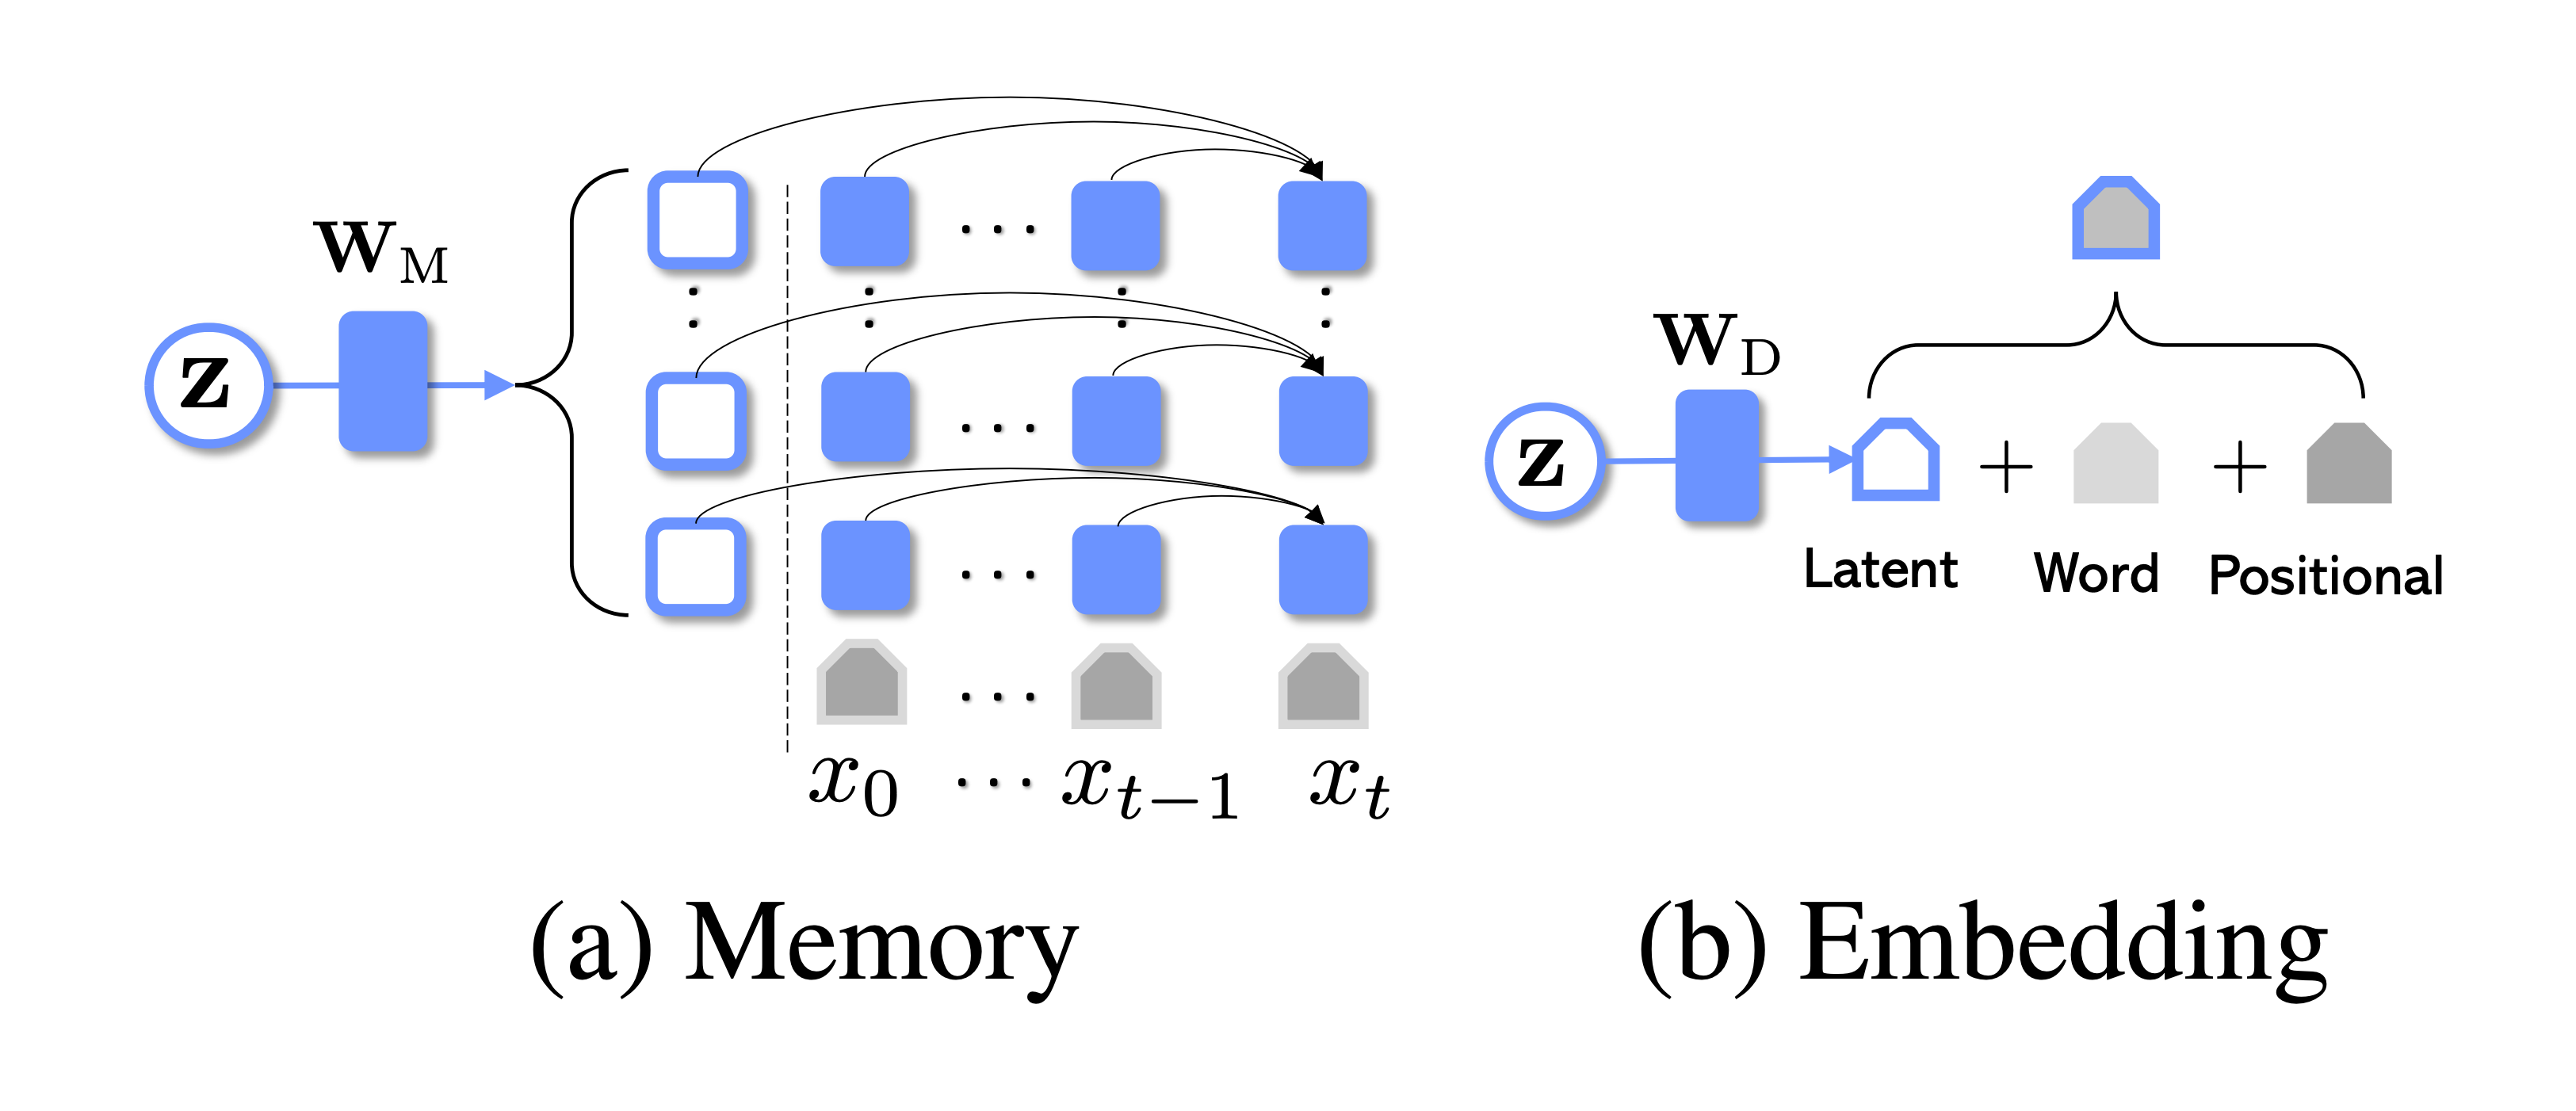
\includegraphics[width=8cm]{bilder/latent_optimus}
    \caption{Methoden um den Latentvector in GPT-2 zu injizieren}
    \label{latent_optimus}
\end{figure}

Um mit GPT-2 kontrolliert unter Verwendung des Latentvektors Text zu generieren kann der Latentvektor entweder als Memoryvektor in die Past-Gewichtsmatrix injeziert oder auf die alten Embeddings addiert werden.

Beim Embedding wird $z$ direkt auf den Embedding Layer addiert. Somit ergibt sich der neue Embedding Layer durch $h_{Emb}^{'} = h_{Emb} + W_D z$ mit der Gewichtsmatrix $W_D \in \mathbb{R}^{H \times P}$.
Der Decoder kann hier die zusätzlichen Informationen des Embeddings beim Input und Output Layer verwenden.

Bei der Injezierung von $z$ als Memoryvektor $h_{Mem} \in \mathbb{R}^{L\times H}$ wird der Latentvektor in den Past Key Vektor von GPT-2 injeziert. Der Past Key Vector beschleunigt normalerweise den Decodiervorgang von GPT-2, da bei einem Decodierungsdurchlauf zu den vorherigen Tokens bereits entsprechende Key- und Valuevektoren in den Attentionlayern berechnet wurden.
Diese Key-, Valuevektoren des Attentionlayers werden durch $h_{Mem} = W_M z$ mit $W_M \in \mathbb{R}^{LH \times P}$ ersetzt. GPT-2 kann so beim Decodieren auf den injezierten Latentvektor bei jeder Attentionberechnung zugreifen.

Die Parameter ${\phi_{BERT}, \theta_{GPT-2}, W_E,W_M,W_D}$ des VAEs werden mittels Cyclical Annealing Schedule \citep{DBLP:journals/corr/abs-1903-10145} trainiert, um das KL Vanishing Problem beim Trainieren eines VAEs zu verhindern.
Die $\beta$ Variable, die wie in \ref{cyc_anneal} erklärt den KL Regularisierer Anteil steuert, wird für einen Trainingsdurchlauf für die erste halbe Menge der Trainingsdaten auf $\beta = 0$ gesetzt. Somit wird zu Beginn lediglich ein Autoencoder trainiert. 
Anschließend wird für das nächste viertel der Trainingsmenge schrittweise $\beta$ von 0 auf 1 erhöht und für das letzte viertel der Trainingsmenge auf 1 belassen um das VAE Model zu trainieren.

Insgesamt zeigt Optimus gute Ergebnisse in den Bereichen des Language Modeling, Kontrollierte Text Generation und Language Understanding.




\subsection{Latent Space Operations}

\pagebreak
